\documentclass{exercise}

\institute{Applied and Computational Mathematics}
\title{Hausaufgabenübung 4}
\author{Joshua Feld, 406718}
\course{Mathematische Grundlagen IV}
\professor{Torrilhon \& Berkels}
\semester{Sommersemester 2022}
\program{CES (Bachelor)}

\begin{document}
    \maketitle


    \section*{Aufgabe 1}

    \begin{problem}
        Bestimmen Sie die Lösung \(u \in C^2\parentheses*{\Omega}\) der Poisson-Gleichung
        \begin{align*}
            -\Delta u\parentheses*{x, y} &= 1, \quad \parentheses*{x, y} \in \Omega,\\
            u\parentheses*{x, y} &= 0, \quad \parentheses*{x, y} \in \partial\Omega,
        \end{align*}
        wobei \(\Omega \subset \R^2\) eine Kreisscheibe mit dem Ursprung als Mittelpunkt und Radius \(R\) ist.
        Gehen Sie dabei wie folgt vor:
        \begin{enumerate}
            \item Transformieren Sie zuerst auf Polarkoordinaten und nutzen Sie dann, dass die Lösung rotationssymmetrisch, d.h. winkelunabhängig ist, also
            \[
                u\parentheses*{r\cos\phi, r\sin\phi} = v\parentheses*{r}.
            \]
            Zeigen Sie, dass sich dabei die Differentialgleichung
            \begin{equation}\label{eq:1}
                v''\parentheses*{r} + \frac{1}{r}v'\parentheses*{r} + 1 = 0
            \end{equation}
            ergibt.
            \item Weisen Sie nach, dass die Funktion
            \[
                f\parentheses*{x} = \frac{c}{x} - \frac{x}{2}, \quad c \in \R
            \]
            die Differentialgleichung
            \[
                f'\parentheses*{x} + \frac{f\parentheses*{x}}{x} + 1 = 0
            \]
            löst und bestimmen Sie die allgemeine Lösung der Differentialgleichung \eqref{eq:1}.
        \end{enumerate}
    \end{problem}

    \subsection*{Lösung}
    \begin{enumerate}
        \item Aufgrund der Rotationssymmetrie ist \(u\parentheses*{r\sin\phi, r\cos\phi}\) winkelunabhängig.
        Geht man auf Polarkoordinaten über, ergibt sich mit \(u\parentheses*{r\cos\phi, r\sin\phi} = v\parentheses*{r}\)
        \begin{align*}
            \Delta u = \parentheses*{\frac{\partial^2}{\partial r^2} + \frac{1}{r^2}\frac{\partial^2}{\partial\phi^2} + \frac{1}{r}\frac{\partial}{\partial r}}v\parentheses*{r} &= -1,\\
            \frac{\partial^2 v}{\partial r^2} + \frac{1}{r}\frac{\partial v}{\partial r} &= -1.
        \end{align*}
        \item Wir lösen
        \[
            f' + \frac{f}{x} + 1 = 0.
        \]
        \begin{enumerate}
            \item Lösen der homogenen Differentialgleichung \(f' = -\frac{f}{x}\) durch Trennen der Variablen ergibt
            \[
                \int\frac{f'}{f}\d x = -\int\frac{1}{x}\dx + k \iff \ln f = -\ln x + k, \quad k \in \R,
            \]
            also
            \[
                f\parentheses*{x} = e^k e^{-\ln x} = \frac{c}{x}, \quad c \in \R.
            \]
            \item Lösen der inhomogenen Differentialgleichung mit Variation der Konstanten \(f\parentheses*{x} = \frac{c\parentheses*{x}}{x}\).
            Einsetzen in die Differentialgleichung \(f' + \frac{f}{x} + 1 = 0\) liefert
            \[
                \frac{c'\parentheses*{x}}{x} - \frac{c\parentheses*{x}}{x^2} + \frac{c\parentheses*{x}}{x^2} + 1 = 0 \iff c'\parentheses*{x} = -x \iff c\parentheses*{x} = -\frac{x^2}{x} - \gamma, \quad \gamma \in \R.
            \]
            Die allgemeine Lösung der Differentialgleichung ist also
            \[
                f\parentheses*{x} = \parentheses*{\gamma - \frac{x^2}{2}}\frac{1}{x} = \frac{\gamma}{x} - \frac{x}{2}.
            \]
            Vergleicht man jetzt die Differentialgleichung \(v'' + \frac{1}{r}v' + 1 = 0\) mit der angegebenen, so entspricht \(x\) den \(r\) und \(v'\) entspricht \(f\), d.h. für \(v\) gilt
            \[
                v'\parentheses*{r} = \frac{\gamma}{r} - \frac{r}{2} \iff v\parentheses*{r} = \gamma\ln r - \frac{r^2}{4} + \beta, \quad \beta, \gamma \in \R.
            \]
        \end{enumerate}
        Da \(u \in C^2\parentheses*{\Omega}\) sein muss, folgt direkt, dass \(\gamma = 0\) ist (ansonsten wäre \(u\parentheses*{0, 0}\) nicht definiert).
        Aus der Randbedingung \(u = 0\) auf \(\partial\Omega\) folgt \(v\parentheses*{R} = 0\) bzw.
        \[
            -\frac{R^2}{4} + \beta = 0 \quad \text{oder} \quad \beta = \frac{R^2}{4}.
        \]
        Man erhält also \(v\parentheses*{r} = \frac{r^2 - R^2}{4}\) bzw. \(u\parentheses*{x, y} = \frac{x^2 + y^2 - R^2}{4}\).
        Da das Problem auch für den Kreisring rotationssymmetrisch bzw. winkelunabhängig ist, gilt ebenfalls \(u\parentheses*{r\cos\phi, r\sin\phi} = v\parentheses*{r}\).
        Wir erhalten daher die gleiche allgemeine Lösung
        \[
            v\parentheses*{r} = \gamma\ln r - \frac{r^2}{4} + \beta, \quad \beta, \gamma \in \R.
        \]
        Aus den Randbedingungen folgt jetzt
        \begin{align*}
            0 &= v\parentheses*{R_i} = \gamma\ln R_i - \frac{R_i^2}{4} + \beta,\\
            0 &= v\parentheses*{R_a} = \gamma\ln R_a - \frac{R_a^2}{4} + \beta.
        \end{align*}
        Subtraktion der beiden GLeichungen liefert \(\gamma\parentheses*{\ln R_i - \ln R_a} = \frac{R_i^2 - R_a^2}{4}\), also
        \[
            \gamma = \frac{R_i^2 - R_a^2}{4\parentheses*{\ln R_i - \ln R_a}}.
        \]
        Damit ist
        \[
            \beta = \frac{R_i^2}{4} - \gamma\ln R_i = \frac{R_a^2 \ln R_i - R_i^2 \ln R_a}{4\parentheses*{\ln R_i - \ln R_a}}.
        \]
        Also gilt für die Lösung
        \[
            v\parentheses*{r} = \frac{1}{4}\parentheses*{\frac{R_i^2 - R_a^2}{\ln R_i - \ln R_a}\ln r - r^2 + \frac{R_a^2 \ln R_i - R_i^2 \ln R_a}{\ln R_i - \ln R_a}}.
        \]
    \end{enumerate}


    \section*{Aufgabe 2}

    \begin{problem}
        In dieser Aufgabe betrachten wir finite Differenzen-Approximationen höherer Approximationsordnung.
        Für die Approximation der zweiten Ableitung von \(f \in C^6\parentheses*{\Omega}\) sei eine finite Differenz mit folgenden Parametern gegeben:
        \[
            \bm{h} = h\parentheses*{-2, -1, 0, 1, 2}, \quad \bm{\alpha} = \frac{1}{h^2}\parentheses*{a_{-2}, a_{-1}, a_0, a_1, a_2}.
        \]
        Bestimmen Sie \(a_i, i = -2, \ldots, 2\) so, dass der Approximationsfehler der Ordnung \(\mathcal{O}\parentheses*{h^4}\) ist.
    \end{problem}

    \subsection*{Lösung}
    Der Differenzenstern gibt uns
    \[
        \frac{1}{h^2}\parentheses*{a_{-2}f\parentheses*{x - 2h} + a_{-1}f\parentheses*{x - h} + a_0 f\parentheses*{x} + a_1 f\parentheses*{x + h} + a_2 f\parentheses*{x + 2h}}.
    \]
    Eine Taylorentwicklung gobt uns folgende Terme in folgenden Ordnungen:
    \begin{align*}
        \mathcal{O}\parentheses*{h^{-2}}: &\quad \parentheses*{a_{-2} + a_{-1} + a_0 + a_1 + a_2}f\parentheses*{x},\\
        \mathcal{O}\parentheses*{h^{-1}}: &\quad \parentheses*{-2a_{-2} - a_{-1} + a_1 + 2a_2}f'\parentheses*{x},\\
        \mathcal{O}\parentheses*{h^0}: &\quad \parentheses*{2a_{-2} + \frac{a_{-1}}{2} + \frac{a_1}{2} + 2a_2}f''\parentheses*{x},\\
        \mathcal{O}\parentheses*{h^1}: &\quad \parentheses*{-\frac{4a_{-2}}{3} - \frac{a_{-1}}{6} + \frac{a_1}{6} + \frac{4a_2}{3}}f^{\parentheses*{3}}\parentheses*{x},\\
        \mathcal{O}\parentheses*{h^2}: &\quad \parentheses*{\frac{2a_{-2}}{3} + \frac{a_{-1}}{24} + \frac{a_1}{24} + \frac{2a_2}{3}}f^{\parentheses*{4}}\parentheses*{x},\\
        \mathcal{O}\parentheses*{h^3}: &\quad \parentheses*{-\frac{4a_{-2}}{15} - \frac{a_{-1}}{120} + \frac{a_1}{120} + \frac{4a_2}{15}}f^{\parentheses*{5}}\parentheses*{x},\\
        \mathcal{O}\parentheses*{h^4}: &\quad \parentheses*{\frac{4a_{-2}}{45} + \frac{a_{-1}}{720} + \frac{a_1}{720} + \frac{4a_2}{45}}f^{\parentheses*{6}}\parentheses*{x}.
    \end{align*}
    Um Ordnung \(\mathcal{O}\parentheses*{h^4}\) benötigen wir, dass die Terme der Ordnungen \(\mathcal{O}\parentheses*{h^k}, k \in \braces*{-2, -1, 1, 2, 3}\) verschwinden und der Term der Ordnung \(\mathcal{O}\parentheses*{1}\) muss \(f''\parentheses*{x}\) entsprechen.
    Wir können dies als lineares Problem schreiben:
    \[
        \begin{pmatrix}
            1 & 1 & 1 & 1 & 1\\
            -2 & -1 & 0 & 1 & 2\\
            2 & \frac{1}{2} & 0 & \frac{1}{2} & 2\\
            -\frac{4}{3} & -\frac{1}{6} & 0 & \frac{1}{6} & \frac{4}{3}\\
            \frac{2}{3} & \frac{1}{24} & 0 & \frac{1}{24} & \frac{2}{3}\\
            -\frac{4}{15} & -\frac{1}{120} & 0 & \frac{1}{120} & \frac{4}{15}
        \end{pmatrix}\begin{pmatrix}
            a_{-2}\\a_{-1}\\a_0\\a_1\\a_2
        \end{pmatrix} = \begin{pmatrix}
            0\\0\\1\\0\\0\\0
        \end{pmatrix}.
    \]
    Wir finden die Lösung
    \[
        a_{-2} = -\frac{1}{12}, \quad a_{-1} = \frac{4}{3}, \quad a_0 = -\frac{5}{2}, \quad a_1 = \frac{4}{3}, \quad a_2 = -\frac{1}{12}.
    \]
    Mit dieser Lösung erhalten wir
    \[
        \frac{1}{h^2}\parentheses*{a_{-2}f\parentheses*{x - 2h} + a_{-1}f\parentheses*{x - h} + a_0 f\parentheses*{x} + a_1 f\parentheses*{x + h} + a_2 f\parentheses*{x + 2h}} = f''\parentheses*{x} - \frac{1}{90}h^4 f^{\parentheses*{6}} + \mathcal{O}\parentheses*{h^7}.
    \]
    Damit ist die Approximation vierter Ordnung.


    \section*{Aufgabe 3}

    \begin{problem}
        In dieser Aufgabe sollen Gleichungssysteme für die Diskretisierung der Poissongleichung mit verschiedenen Anordnungen der Gitterpunkte aufgestellt werden.
        Diskretisieren Sie auf \(\Omega = \parentheses*{0, 1} \times \parentheses*{0, 1}\) die Gleichung
        \begin{align*}
            -\Delta u\parentheses*{x, y} &= f\parentheses*{x, y}, \quad \parentheses*{x, y} \in \Omega,\\
            u\parentheses*{x, y} &= 0, \quad \parentheses*{x, y} \in \partial\Omega,
        \end{align*}
        mit der Differenzenformel
        \[
            \parentheses*{-\Delta_h u}\parentheses*{x, y} = \frac{-u\parentheses*{x - h, y} - u\parentheses*{x + h, y} + 4u\parentheses*{x, y} - u\parentheses*{x, y + h} - u\parentheses*{x, y - h}}{h^2}
        \]
        für \(h = \frac{1}{4}\).
        Stellen Sie hierzu das Gleichungssystem \(Au_h = b\) für folgende Nummerierungen auf:
        \begin{center}
            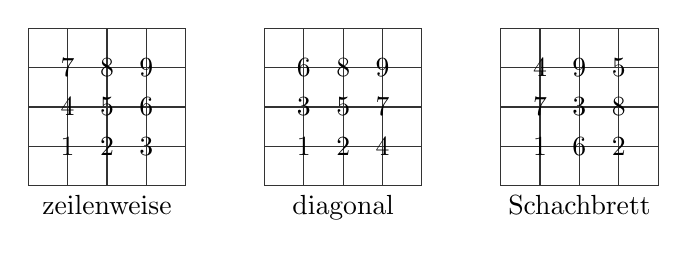
\begin{tikzpicture}
                \draw[color=white!20!black] (0,0) rectangle (2,2);
                \draw[color=white!20!black] (.5,0) -- (.5,2);
                \draw[color=white!20!black] (1,0) -- (1,2);
                \draw[color=white!20!black] (1.5,0) -- (1.5,2);
                \draw[color=white!20!black] (0,.5) -- (2,.5);
                \draw[color=white!20!black] (0,1) -- (2,1);
                \draw[color=white!20!black] (0,1.5) -- (2,1.5);
                \node at (.5,.5) {\(\bm{1}\)};
                \node at (1,.5) {\(\bm{2}\)};
                \node at (1.5,.5) {\(\bm{3}\)};
                \node at (.5,1) {\(\bm{4}\)};
                \node at (1,1) {\(\bm{5}\)};
                \node at (1.5,1) {\(\bm{6}\)};
                \node at (.5,1.5) {\(\bm{7}\)};
                \node at (1,1.5) {\(\bm{8}\)};
                \node at (1.5,1.5) {\(\bm{9}\)};
                \node[anchor=north] at (1,0) {zeilenweise};

                \begin{scope}[shift={(3,0)}]
                    \draw[color=white!20!black] (0,0) rectangle (2,2);
                    \draw[color=white!20!black] (.5,0) -- (.5,2);
                    \draw[color=white!20!black] (1,0) -- (1,2);
                    \draw[color=white!20!black] (1.5,0) -- (1.5,2);
                    \draw[color=white!20!black] (0,.5) -- (2,.5);
                    \draw[color=white!20!black] (0,1) -- (2,1);
                    \draw[color=white!20!black] (0,1.5) -- (2,1.5);
                    \node at (.5,.5) {\(\bm{1}\)};
                    \node at (1,.5) {\(\bm{2}\)};
                    \node at (1.5,.5) {\(\bm{4}\)};
                    \node at (.5,1) {\(\bm{3}\)};
                    \node at (1,1) {\(\bm{5}\)};
                    \node at (1.5,1) {\(\bm{7}\)};
                    \node at (.5,1.5) {\(\bm{6}\)};
                    \node at (1,1.5) {\(\bm{8}\)};
                    \node at (1.5,1.5) {\(\bm{9}\)};
                    \node[anchor=north] at (1,0) {diagonal};
                \end{scope}

                \begin{scope}[shift={(6,0)}]
                    \draw[color=white!20!black] (0,0) rectangle (2,2);
                    \draw[color=white!20!black] (.5,0) -- (.5,2);
                    \draw[color=white!20!black] (1,0) -- (1,2);
                    \draw[color=white!20!black] (1.5,0) -- (1.5,2);
                    \draw[color=white!20!black] (0,.5) -- (2,.5);
                    \draw[color=white!20!black] (0,1) -- (2,1);
                    \draw[color=white!20!black] (0,1.5) -- (2,1.5);
                    \node at (.5,.5) {\(\bm{1}\)};
                    \node at (1,.5) {\(\bm{6}\)};
                    \node at (1.5,.5) {\(\bm{2}\)};
                    \node at (.5,1) {\(\bm{7}\)};
                    \node at (1,1) {\(\bm{3}\)};
                    \node at (1.5,1) {\(\bm{8}\)};
                    \node at (.5,1.5) {\(\bm{4}\)};
                    \node at (1,1.5) {\(\bm{9}\)};
                    \node at (1.5,1.5) {\(\bm{5}\)};
                    \node[anchor=north] at (1,0) {Schachbrett};
                \end{scope}
            \end{tikzpicture}
        \end{center}
    \end{problem}

    \subsection*{Lösung}
    Mit \(u_{ij} = u\parentheses*{x_i, y_i}\) und \(f_{ij} = f\parentheses*{x_i, y_j}\) lauten die Gleichungssysteme:
    \begin{itemize}
        \item Zeilenweise Nummerierung:
        \[
            \frac{1}{h^2}\brackets*{\begin{array}{ccc|ccc|ccc}
                4 & -1 & & -1 & & & & &\\
                -1 & 4 & -1 & & -1 & & & &\\
                & -1 & 4 & & & -1 & & &\\
                \hline
                -1 & & & 4 & -1 & & -1 & &\\
                & -1 & & -1 & 4 & -1 & & -1 &\\
                & & -1 & & -1 & 4 & & & -1\\
                \hline
                & & & -1 & & 4 & -1 &\\
                & & & & -1 & & -1 & 4 & -1\\
                & & & & & -1 & & -1 & 4
            \end{array}}\begin{pmatrix}
                u_{11}\\u_{21}\\u_{31}\\u_{12}\\u_{22}\\u_{32}\\u_{13}\\u_{23}\\u_{33}
            \end{pmatrix} = \begin{pmatrix}
                f_{11}\\f_{21}\\f_{31}\\f_{12}\\f_{22}\\f_{32}\\f_{13}\\f_{23}\\f_{33}
            \end{pmatrix}
        \]
        \item Diagonale Nummerierung:
        \[
            \frac{1}{h^2}\brackets*{\begin{array}{c|cc|ccc|cc|c}
                4 & -1 & -1 & & & & & &\\
                \hline
                -1 & 4 & & -1 & -1 & & & &\\
                -1 & & 4 & & -1 & -1 & & &\\
                \hline
                & -1 & & 4 & & & -1 & &\\
                & -1 & -1 & & 4 & & -1 & -1 &\\
                & & -1 & & & 4 & & -1 &\\
                \hline
                & & & -1 & -1 & & 4 & & -1\\
                & & & & -1 & -1 & & 4 & -1\\
                \hline
                & & & & & & -1 & -1 & 4
            \end{array}}\begin{pmatrix}
                u_{11}\\u_{21}\\u_{31}\\u_{12}\\u_{22}\\u_{32}\\u_{13}\\u_{23}\\u_{33}
            \end{pmatrix} = \begin{pmatrix}
                f_{11}\\f_{21}\\f_{31}\\f_{12}\\f_{22}\\f_{32}\\f_{13}\\f_{23}\\f_{33}
            \end{pmatrix}
        \]
        \item Schachbrett-Nummerierung:
        \[
            \frac{1}{h^2}\brackets*{\begin{array}{ccccc|cccc}
                4 & & & & & -1 & -1 & &\\
                & 4 & & & & -1 & & -1 &\\
                & & 4 & & & -1 & -1 & -1 & -1\\
                & & & 4 & & & -1 & & -1\\
                & & & & 4 & & & -1 & -1\\
                \hline
                -1 & -1 & -1 & & & 4 & & &\\
                -1 & & -1 & -1 & & & 4 & &\\
                & -1 & -1 & & -1 & & & 4 &\\
                & & -1 & -1 & -1 & & & & 4
            \end{array}}\begin{pmatrix}
                u_{11}\\u_{21}\\u_{31}\\u_{12}\\u_{22}\\u_{32}\\u_{13}\\u_{23}\\u_{33}
            \end{pmatrix} = \begin{pmatrix}
                f_{11}\\f_{21}\\f_{31}\\f_{12}\\f_{22}\\f_{32}\\f_{13}\\f_{23}\\f_{33}
            \end{pmatrix}
        \]
    \end{itemize}
\end{document}
